\section{Project implementations}

The project implementation is divided in several sections, where each section
is described. First we've got an overall description of the project which we've
implemented.

\subsection{Overall description}
\begin{figure}[htbp]
   \centering
   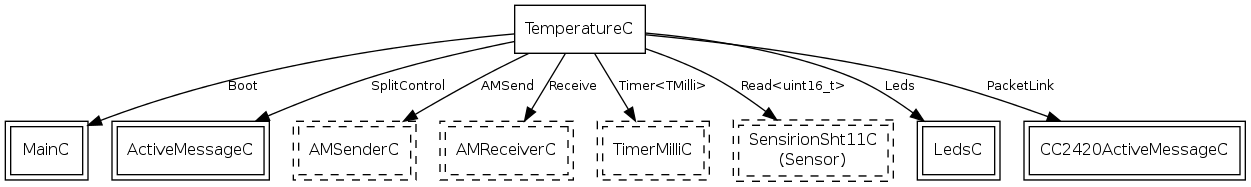
\includegraphics[width=17cm]{img/TemperatureAppC.png} 
   \caption{An overall illustration of the project implmented}
   \label{fig:overalloverview}
\end{figure}

\subsection{Temperature measuring}
Here we'll explain how and where we convert the digital readout from the
temperature sensor to actual degress. The conversion given a digital readout
($SO_{T}$) to a temperature value is given at the following
formula\cite{temperature}:

\begin{align*}
	T &= d_{1} + d_{2} \cdot SO_{T}
\end{align*}
where the coefficients is defined in Tabel ~\ref{table:temperature}
\begin{table}[ht]
\centering
\begin{tabular}{ | l | c | r | }
	\hline
	VDD & $d_{1} \ ^{\circ}  C$ & $d_{1} \ ^{\circ}  F$ \\
	\hline \hline
	5V & -40.1 & -40.2 \\
	\hline
	4V & -39.8 & -39.6 \\
	\hline
	3.5V & -39.7 & -39.5 \\
	\hline
	3V & -39.6 & -39.3 \\
	\hline
	2.5V & -39.4 & -38.9 \\
	\hline
\end{tabular}
\begin{tabular}{ | l | c | r | }
	\hline
	$SO_{T}$ & $d_{2}  \ ^{\circ}C$ & $d_{2} \ ^{\circ} F$ \\
	\hline \hline
	14 bit & 0.01 & 0.018 \\
	\hline
	12 bit & 0.04 & 0.072\\
	\hline
\end{tabular}
\caption{Temperature conversion coefficients}
\label{table:temperature}
\end{table}
The conversion from a digital readout is being done in the event readDone.
We've made two compile time constants, $CONVERSION_{D1}$, and
$CONVERSION_{D2}$.

\begin{lstlisting}
CONVERSION_D1 = 3960, /* VDD = 3V */
CONVERSION_D2 = 1 /* 14 bits */
...
event void Read.readDone(error_t result, uint16_t data) {
	float tempC;
	if (result != SUCCESS){
		data = 0xffff;
		report_problem();
	}
	  // conversion
	  tempC = ( (-CONVERSION_D1) + (CONVERSION_D2 * data) ) ;
    local.readings[reading++] = tempC;
}
\end{lstlisting}


\subsection{Network communication}

\begin{lstlisting}
message_t* receive(message_t *msg, void *payload, uint8_t len) {
		message_t *ret = msg;
		int avg = 0, i = 0;

		if (len == sizeof(temperature_t)) {
			temperature_t* tmpptr = (temperature_t*)payload;
			printf("\n---------------------------\n");
			for (i = 0; i < NREADINGS ; i++) {
				avg = avg + tmpptr->readings[i];
				printf("%d %d \n", tmpptr->count*10 + i, tmpptr->readings[i]);
			}
			avg = avg / NREADINGS;
			printf("average: %d\n", avg);
			printfflush();
			if (avg <= 2800) {
				call Leds.led1Off();
				call Leds.led0On();
			} else {
				call Leds.led0Off();
				call Leds.led1On();
			}
		}
\end{lstlisting}

\subsection{UART / PC Communication}
skriv om brug af printf

\subsection{Acknowledgement}
skriv om hardware/software ACK
